    \documentclass{beamer}
        
        \usepackage{pgf}
        \usepackage{tikz}
        \usepackage{amsmath, amssymb}
        \usetikzlibrary{arrows.meta}
        \usetikzlibrary{arrows}
        \usetikzlibrary{calc}
        \usetikzlibrary{shapes}
        \usepackage[utf8]{inputenc}
        \usetheme{default}
        \usefonttheme{professionalfonts}
        \setbeamertemplate{navigation symbols}{}
        \setbeamerfont{frametitle}{series=\bfseries}
    
        \begin{document}
        
        \begin{frame}
        \frametitle{Breadth-First Traversal : Input}
        \begin{center}
        
        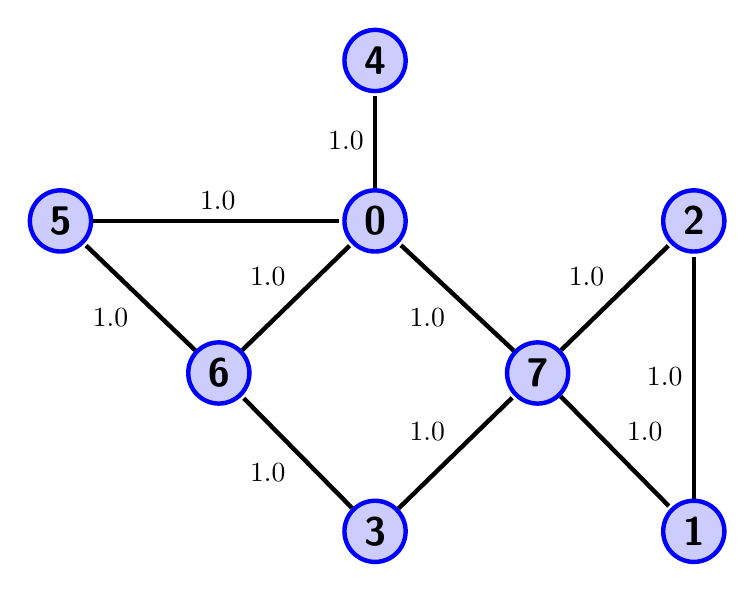
\begin{tikzpicture}[shorten >=1pt, auto, node distance=3cm, ultra thick,
        node_style/.style={circle,draw=blue,fill=blue!20!,font=\sffamily\Large\bfseries},
        selected_node_style/.style={circle,draw=blue,fill=yellow!20!,font=\sffamily\Large\bfseries},
        edge_style/.style={draw=black, ultra thick,-},
        selected_edge_style/.style={draw=yellow, ultra thick,-}]
        
        \node [node_style](n1) at (8.44,7.474) {0};
        \node [node_style](n2) at (12.488,3.532) {1};
        \node [node_style](n3) at (12.488,7.474) {2};
        \node [node_style](n4) at (8.44,3.532) {3};
        \node [node_style](n5) at (8.44,9.512) {4};
        \node [node_style](n6) at (4.445,7.474) {5};
        \node [node_style](n7) at (6.456,5.543) {6};
        \node [node_style](n8) at (10.505,5.543) {7};
        \draw [edge_style] (n4) edge node{1.0} (n7);
        \draw [edge_style] (n2) edge node{1.0} (n3);
        \draw [edge_style] (n7) edge node{1.0} (n1);
        \draw [edge_style] (n8) edge node{1.0} (n1);
        \draw [edge_style] (n4) edge node{1.0} (n8);
        \draw [edge_style] (n1) edge node{1.0} (n5);
        \draw [edge_style] (n8) edge node{1.0} (n3);
        \draw [edge_style] (n7) edge node{1.0} (n6);
        \draw [edge_style] (n6) edge node{1.0} (n1);
        \draw [edge_style] (n8) edge node{1.0} (n2);
        \end{tikzpicture}
    
        \end{center}
        \end{frame}
        
            \begin{frame}
            \frametitle{Breadth-First Traversal Iteration:1 Queue:[3]}
            
        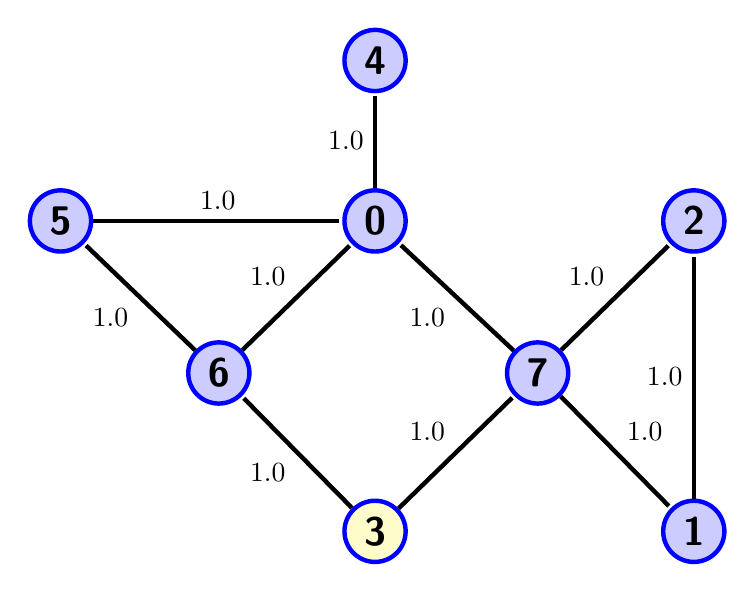
\begin{tikzpicture}[shorten >=1pt, auto, node distance=3cm, ultra thick,
        node_style/.style={circle,draw=blue,fill=blue!20!,font=\sffamily\Large\bfseries},
        selected_node_style/.style={circle,draw=blue,fill=yellow!20!,font=\sffamily\Large\bfseries},
        edge_style/.style={draw=black, ultra thick,-},
        selected_edge_style/.style={draw=yellow, ultra thick,-}]
        
        \node [node_style](n1) at (8.44,7.474) {0};
        \node [node_style](n2) at (12.488,3.532) {1};
        \node [node_style](n3) at (12.488,7.474) {2};
        \node [selected_node_style](n4) at (8.44,3.532) {3};
        \node [node_style](n5) at (8.44,9.512) {4};
        \node [node_style](n6) at (4.445,7.474) {5};
        \node [node_style](n7) at (6.456,5.543) {6};
        \node [node_style](n8) at (10.505,5.543) {7};
        \draw [edge_style] (n4) edge node{1.0} (n7);
        \draw [edge_style] (n2) edge node{1.0} (n3);
        \draw [edge_style] (n7) edge node{1.0} (n1);
        \draw [edge_style] (n8) edge node{1.0} (n1);
        \draw [edge_style] (n4) edge node{1.0} (n8);
        \draw [edge_style] (n1) edge node{1.0} (n5);
        \draw [edge_style] (n8) edge node{1.0} (n3);
        \draw [edge_style] (n7) edge node{1.0} (n6);
        \draw [edge_style] (n6) edge node{1.0} (n1);
        \draw [edge_style] (n8) edge node{1.0} (n2);
        \end{tikzpicture}
    
            \end{frame}
        
            \begin{frame}
            \frametitle{Breadth-First Traversal Iteration:2 Queue:[6]}
            
        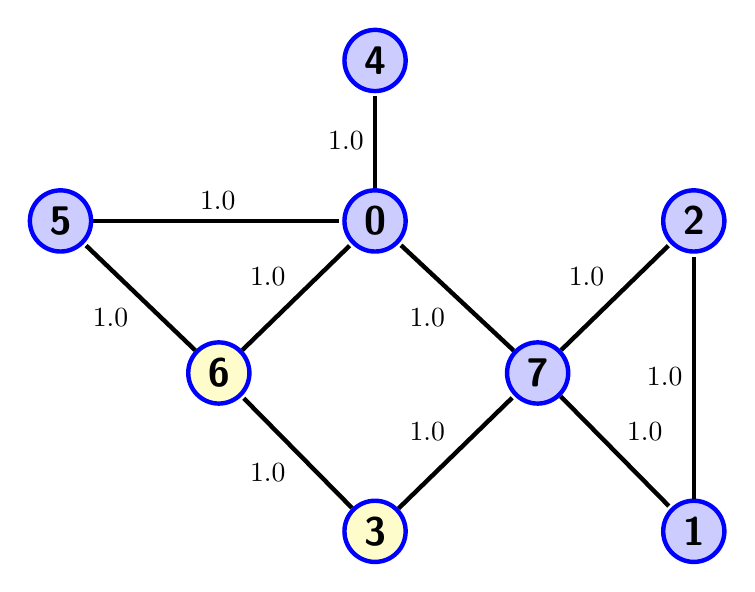
\begin{tikzpicture}[shorten >=1pt, auto, node distance=3cm, ultra thick,
        node_style/.style={circle,draw=blue,fill=blue!20!,font=\sffamily\Large\bfseries},
        selected_node_style/.style={circle,draw=blue,fill=yellow!20!,font=\sffamily\Large\bfseries},
        edge_style/.style={draw=black, ultra thick,-},
        selected_edge_style/.style={draw=yellow, ultra thick,-}]
        
        \node [node_style](n1) at (8.44,7.474) {0};
        \node [node_style](n2) at (12.488,3.532) {1};
        \node [node_style](n3) at (12.488,7.474) {2};
        \node [selected_node_style](n4) at (8.44,3.532) {3};
        \node [node_style](n5) at (8.44,9.512) {4};
        \node [node_style](n6) at (4.445,7.474) {5};
        \node [selected_node_style](n7) at (6.456,5.543) {6};
        \node [node_style](n8) at (10.505,5.543) {7};
        \draw [edge_style] (n4) edge node{1.0} (n7);
        \draw [edge_style] (n2) edge node{1.0} (n3);
        \draw [edge_style] (n7) edge node{1.0} (n1);
        \draw [edge_style] (n8) edge node{1.0} (n1);
        \draw [edge_style] (n4) edge node{1.0} (n8);
        \draw [edge_style] (n1) edge node{1.0} (n5);
        \draw [edge_style] (n8) edge node{1.0} (n3);
        \draw [edge_style] (n7) edge node{1.0} (n6);
        \draw [edge_style] (n6) edge node{1.0} (n1);
        \draw [edge_style] (n8) edge node{1.0} (n2);
        \end{tikzpicture}
    
            \end{frame}
        
            \begin{frame}
            \frametitle{Breadth-First Traversal Iteration:3 Queue:[6,7]}
            
        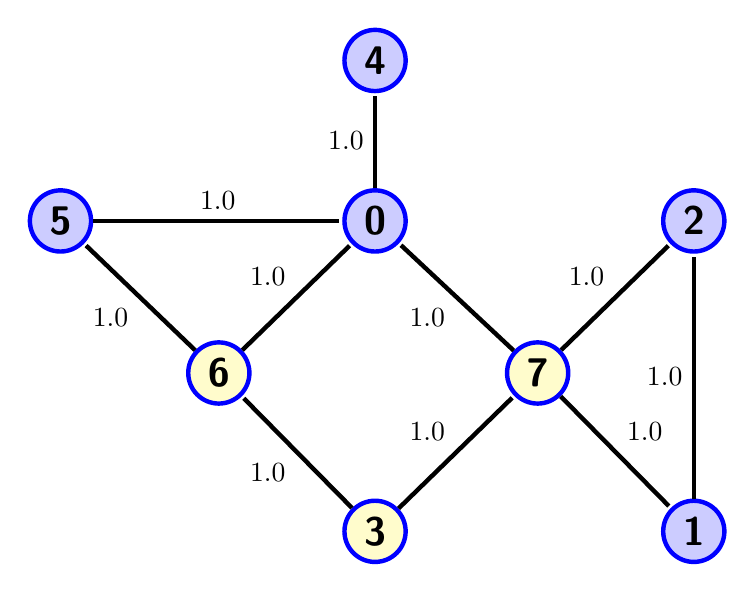
\begin{tikzpicture}[shorten >=1pt, auto, node distance=3cm, ultra thick,
        node_style/.style={circle,draw=blue,fill=blue!20!,font=\sffamily\Large\bfseries},
        selected_node_style/.style={circle,draw=blue,fill=yellow!20!,font=\sffamily\Large\bfseries},
        edge_style/.style={draw=black, ultra thick,-},
        selected_edge_style/.style={draw=yellow, ultra thick,-}]
        
        \node [node_style](n1) at (8.44,7.474) {0};
        \node [node_style](n2) at (12.488,3.532) {1};
        \node [node_style](n3) at (12.488,7.474) {2};
        \node [selected_node_style](n4) at (8.44,3.532) {3};
        \node [node_style](n5) at (8.44,9.512) {4};
        \node [node_style](n6) at (4.445,7.474) {5};
        \node [selected_node_style](n7) at (6.456,5.543) {6};
        \node [selected_node_style](n8) at (10.505,5.543) {7};
        \draw [edge_style] (n4) edge node{1.0} (n7);
        \draw [edge_style] (n2) edge node{1.0} (n3);
        \draw [edge_style] (n7) edge node{1.0} (n1);
        \draw [edge_style] (n8) edge node{1.0} (n1);
        \draw [edge_style] (n4) edge node{1.0} (n8);
        \draw [edge_style] (n1) edge node{1.0} (n5);
        \draw [edge_style] (n8) edge node{1.0} (n3);
        \draw [edge_style] (n7) edge node{1.0} (n6);
        \draw [edge_style] (n6) edge node{1.0} (n1);
        \draw [edge_style] (n8) edge node{1.0} (n2);
        \end{tikzpicture}
    
            \end{frame}
        
            \begin{frame}
            \frametitle{Breadth-First Traversal Iteration:4 Queue:[7,0]}
            
        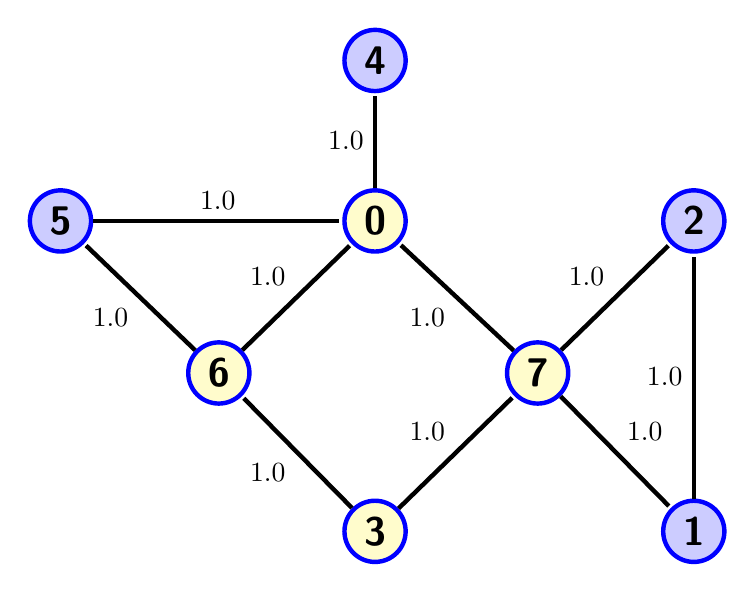
\begin{tikzpicture}[shorten >=1pt, auto, node distance=3cm, ultra thick,
        node_style/.style={circle,draw=blue,fill=blue!20!,font=\sffamily\Large\bfseries},
        selected_node_style/.style={circle,draw=blue,fill=yellow!20!,font=\sffamily\Large\bfseries},
        edge_style/.style={draw=black, ultra thick,-},
        selected_edge_style/.style={draw=yellow, ultra thick,-}]
        
        \node [selected_node_style](n1) at (8.44,7.474) {0};
        \node [node_style](n2) at (12.488,3.532) {1};
        \node [node_style](n3) at (12.488,7.474) {2};
        \node [selected_node_style](n4) at (8.44,3.532) {3};
        \node [node_style](n5) at (8.44,9.512) {4};
        \node [node_style](n6) at (4.445,7.474) {5};
        \node [selected_node_style](n7) at (6.456,5.543) {6};
        \node [selected_node_style](n8) at (10.505,5.543) {7};
        \draw [edge_style] (n4) edge node{1.0} (n7);
        \draw [edge_style] (n2) edge node{1.0} (n3);
        \draw [edge_style] (n7) edge node{1.0} (n1);
        \draw [edge_style] (n8) edge node{1.0} (n1);
        \draw [edge_style] (n4) edge node{1.0} (n8);
        \draw [edge_style] (n1) edge node{1.0} (n5);
        \draw [edge_style] (n8) edge node{1.0} (n3);
        \draw [edge_style] (n7) edge node{1.0} (n6);
        \draw [edge_style] (n6) edge node{1.0} (n1);
        \draw [edge_style] (n8) edge node{1.0} (n2);
        \end{tikzpicture}
    
            \end{frame}
        
            \begin{frame}
            \frametitle{Breadth-First Traversal Iteration:5 Queue:[7,0,5]}
            
        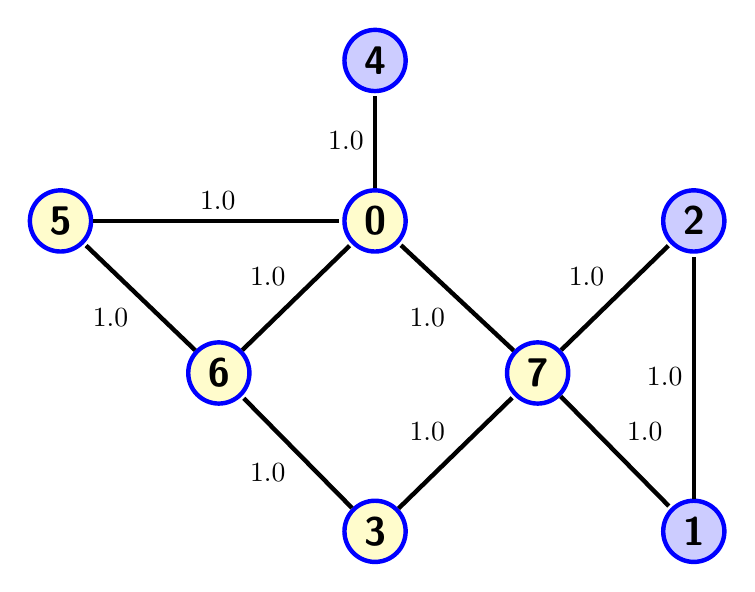
\begin{tikzpicture}[shorten >=1pt, auto, node distance=3cm, ultra thick,
        node_style/.style={circle,draw=blue,fill=blue!20!,font=\sffamily\Large\bfseries},
        selected_node_style/.style={circle,draw=blue,fill=yellow!20!,font=\sffamily\Large\bfseries},
        edge_style/.style={draw=black, ultra thick,-},
        selected_edge_style/.style={draw=yellow, ultra thick,-}]
        
        \node [selected_node_style](n1) at (8.44,7.474) {0};
        \node [node_style](n2) at (12.488,3.532) {1};
        \node [node_style](n3) at (12.488,7.474) {2};
        \node [selected_node_style](n4) at (8.44,3.532) {3};
        \node [node_style](n5) at (8.44,9.512) {4};
        \node [selected_node_style](n6) at (4.445,7.474) {5};
        \node [selected_node_style](n7) at (6.456,5.543) {6};
        \node [selected_node_style](n8) at (10.505,5.543) {7};
        \draw [edge_style] (n4) edge node{1.0} (n7);
        \draw [edge_style] (n2) edge node{1.0} (n3);
        \draw [edge_style] (n7) edge node{1.0} (n1);
        \draw [edge_style] (n8) edge node{1.0} (n1);
        \draw [edge_style] (n4) edge node{1.0} (n8);
        \draw [edge_style] (n1) edge node{1.0} (n5);
        \draw [edge_style] (n8) edge node{1.0} (n3);
        \draw [edge_style] (n7) edge node{1.0} (n6);
        \draw [edge_style] (n6) edge node{1.0} (n1);
        \draw [edge_style] (n8) edge node{1.0} (n2);
        \end{tikzpicture}
    
            \end{frame}
        
            \begin{frame}
            \frametitle{Breadth-First Traversal Iteration:6 Queue:[0,5,1]}
            
        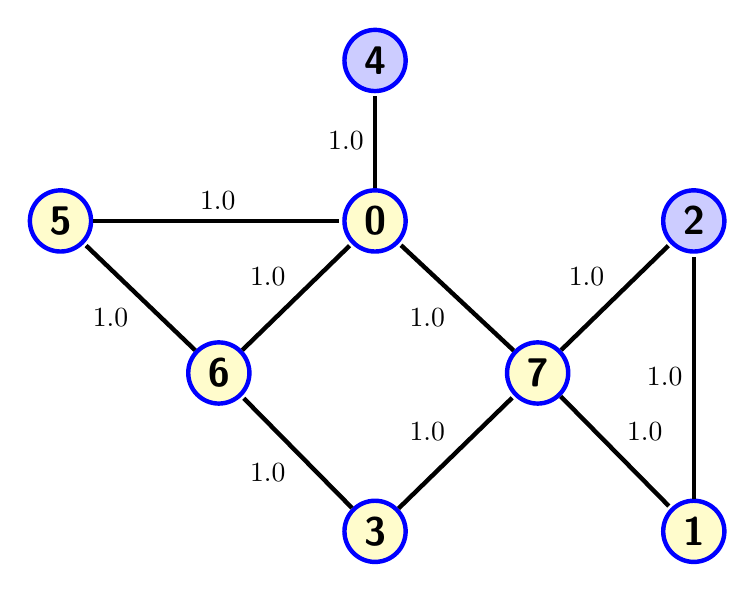
\begin{tikzpicture}[shorten >=1pt, auto, node distance=3cm, ultra thick,
        node_style/.style={circle,draw=blue,fill=blue!20!,font=\sffamily\Large\bfseries},
        selected_node_style/.style={circle,draw=blue,fill=yellow!20!,font=\sffamily\Large\bfseries},
        edge_style/.style={draw=black, ultra thick,-},
        selected_edge_style/.style={draw=yellow, ultra thick,-}]
        
        \node [selected_node_style](n1) at (8.44,7.474) {0};
        \node [selected_node_style](n2) at (12.488,3.532) {1};
        \node [node_style](n3) at (12.488,7.474) {2};
        \node [selected_node_style](n4) at (8.44,3.532) {3};
        \node [node_style](n5) at (8.44,9.512) {4};
        \node [selected_node_style](n6) at (4.445,7.474) {5};
        \node [selected_node_style](n7) at (6.456,5.543) {6};
        \node [selected_node_style](n8) at (10.505,5.543) {7};
        \draw [edge_style] (n4) edge node{1.0} (n7);
        \draw [edge_style] (n2) edge node{1.0} (n3);
        \draw [edge_style] (n7) edge node{1.0} (n1);
        \draw [edge_style] (n8) edge node{1.0} (n1);
        \draw [edge_style] (n4) edge node{1.0} (n8);
        \draw [edge_style] (n1) edge node{1.0} (n5);
        \draw [edge_style] (n8) edge node{1.0} (n3);
        \draw [edge_style] (n7) edge node{1.0} (n6);
        \draw [edge_style] (n6) edge node{1.0} (n1);
        \draw [edge_style] (n8) edge node{1.0} (n2);
        \end{tikzpicture}
    
            \end{frame}
        
            \begin{frame}
            \frametitle{Breadth-First Traversal Iteration:7 Queue:[0,5,1,2]}
            
        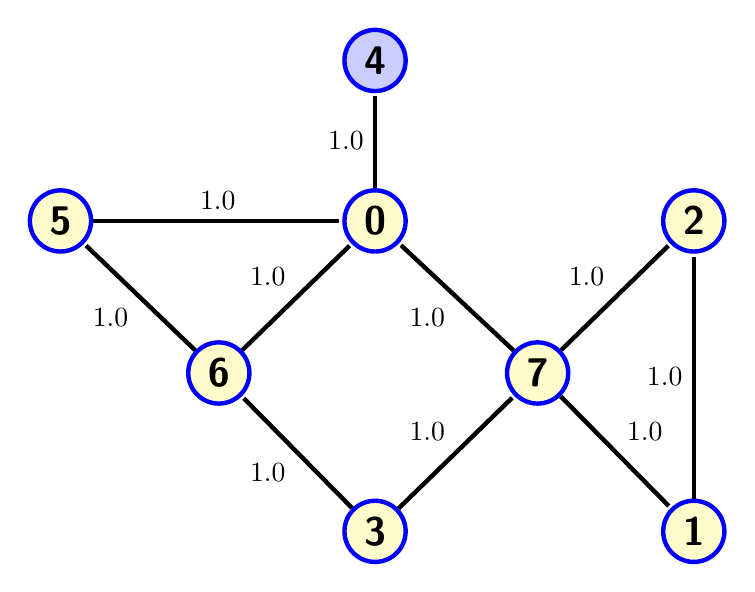
\begin{tikzpicture}[shorten >=1pt, auto, node distance=3cm, ultra thick,
        node_style/.style={circle,draw=blue,fill=blue!20!,font=\sffamily\Large\bfseries},
        selected_node_style/.style={circle,draw=blue,fill=yellow!20!,font=\sffamily\Large\bfseries},
        edge_style/.style={draw=black, ultra thick,-},
        selected_edge_style/.style={draw=yellow, ultra thick,-}]
        
        \node [selected_node_style](n1) at (8.44,7.474) {0};
        \node [selected_node_style](n2) at (12.488,3.532) {1};
        \node [selected_node_style](n3) at (12.488,7.474) {2};
        \node [selected_node_style](n4) at (8.44,3.532) {3};
        \node [node_style](n5) at (8.44,9.512) {4};
        \node [selected_node_style](n6) at (4.445,7.474) {5};
        \node [selected_node_style](n7) at (6.456,5.543) {6};
        \node [selected_node_style](n8) at (10.505,5.543) {7};
        \draw [edge_style] (n4) edge node{1.0} (n7);
        \draw [edge_style] (n2) edge node{1.0} (n3);
        \draw [edge_style] (n7) edge node{1.0} (n1);
        \draw [edge_style] (n8) edge node{1.0} (n1);
        \draw [edge_style] (n4) edge node{1.0} (n8);
        \draw [edge_style] (n1) edge node{1.0} (n5);
        \draw [edge_style] (n8) edge node{1.0} (n3);
        \draw [edge_style] (n7) edge node{1.0} (n6);
        \draw [edge_style] (n6) edge node{1.0} (n1);
        \draw [edge_style] (n8) edge node{1.0} (n2);
        \end{tikzpicture}
    
            \end{frame}
        
            \begin{frame}
            \frametitle{Breadth-First Traversal Iteration:8 Queue:[5,1,2,4]}
            
        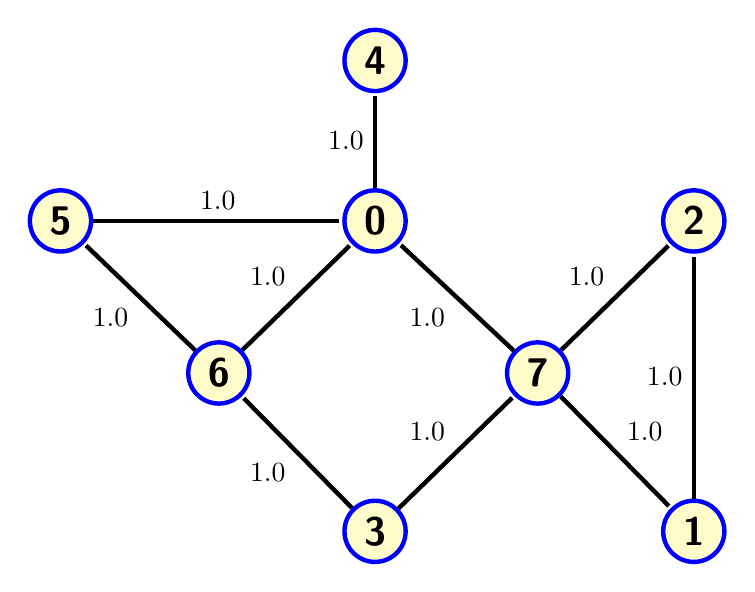
\begin{tikzpicture}[shorten >=1pt, auto, node distance=3cm, ultra thick,
        node_style/.style={circle,draw=blue,fill=blue!20!,font=\sffamily\Large\bfseries},
        selected_node_style/.style={circle,draw=blue,fill=yellow!20!,font=\sffamily\Large\bfseries},
        edge_style/.style={draw=black, ultra thick,-},
        selected_edge_style/.style={draw=yellow, ultra thick,-}]
        
        \node [selected_node_style](n1) at (8.44,7.474) {0};
        \node [selected_node_style](n2) at (12.488,3.532) {1};
        \node [selected_node_style](n3) at (12.488,7.474) {2};
        \node [selected_node_style](n4) at (8.44,3.532) {3};
        \node [selected_node_style](n5) at (8.44,9.512) {4};
        \node [selected_node_style](n6) at (4.445,7.474) {5};
        \node [selected_node_style](n7) at (6.456,5.543) {6};
        \node [selected_node_style](n8) at (10.505,5.543) {7};
        \draw [edge_style] (n4) edge node{1.0} (n7);
        \draw [edge_style] (n2) edge node{1.0} (n3);
        \draw [edge_style] (n7) edge node{1.0} (n1);
        \draw [edge_style] (n8) edge node{1.0} (n1);
        \draw [edge_style] (n4) edge node{1.0} (n8);
        \draw [edge_style] (n1) edge node{1.0} (n5);
        \draw [edge_style] (n8) edge node{1.0} (n3);
        \draw [edge_style] (n7) edge node{1.0} (n6);
        \draw [edge_style] (n6) edge node{1.0} (n1);
        \draw [edge_style] (n8) edge node{1.0} (n2);
        \end{tikzpicture}
    
            \end{frame}
        
    \end{document}
    
